\documentclass[]{book}
\usepackage{lmodern}
\usepackage{amssymb,amsmath}
\usepackage{ifxetex,ifluatex}
\usepackage{fixltx2e} % provides \textsubscript
\ifnum 0\ifxetex 1\fi\ifluatex 1\fi=0 % if pdftex
  \usepackage[T1]{fontenc}
  \usepackage[utf8]{inputenc}
\else % if luatex or xelatex
  \ifxetex
    \usepackage{mathspec}
  \else
    \usepackage{fontspec}
  \fi
  \defaultfontfeatures{Ligatures=TeX,Scale=MatchLowercase}
\fi
% use upquote if available, for straight quotes in verbatim environments
\IfFileExists{upquote.sty}{\usepackage{upquote}}{}
% use microtype if available
\IfFileExists{microtype.sty}{%
\usepackage{microtype}
\UseMicrotypeSet[protrusion]{basicmath} % disable protrusion for tt fonts
}{}
\usepackage[unicode=true]{hyperref}
\hypersetup{
            pdftitle={Applied Linear Models},
            pdfauthor={Nick Syring},
            pdfborder={0 0 0},
            breaklinks=true}
\urlstyle{same}  % don't use monospace font for urls
\usepackage{natbib}
\bibliographystyle{plainnat}
\usepackage{color}
\usepackage{fancyvrb}
\newcommand{\VerbBar}{|}
\newcommand{\VERB}{\Verb[commandchars=\\\{\}]}
\DefineVerbatimEnvironment{Highlighting}{Verbatim}{commandchars=\\\{\}}
% Add ',fontsize=\small' for more characters per line
\usepackage{framed}
\definecolor{shadecolor}{RGB}{248,248,248}
\newenvironment{Shaded}{\begin{snugshade}}{\end{snugshade}}
\newcommand{\KeywordTok}[1]{\textcolor[rgb]{0.13,0.29,0.53}{\textbf{{#1}}}}
\newcommand{\DataTypeTok}[1]{\textcolor[rgb]{0.13,0.29,0.53}{{#1}}}
\newcommand{\DecValTok}[1]{\textcolor[rgb]{0.00,0.00,0.81}{{#1}}}
\newcommand{\BaseNTok}[1]{\textcolor[rgb]{0.00,0.00,0.81}{{#1}}}
\newcommand{\FloatTok}[1]{\textcolor[rgb]{0.00,0.00,0.81}{{#1}}}
\newcommand{\ConstantTok}[1]{\textcolor[rgb]{0.00,0.00,0.00}{{#1}}}
\newcommand{\CharTok}[1]{\textcolor[rgb]{0.31,0.60,0.02}{{#1}}}
\newcommand{\SpecialCharTok}[1]{\textcolor[rgb]{0.00,0.00,0.00}{{#1}}}
\newcommand{\StringTok}[1]{\textcolor[rgb]{0.31,0.60,0.02}{{#1}}}
\newcommand{\VerbatimStringTok}[1]{\textcolor[rgb]{0.31,0.60,0.02}{{#1}}}
\newcommand{\SpecialStringTok}[1]{\textcolor[rgb]{0.31,0.60,0.02}{{#1}}}
\newcommand{\ImportTok}[1]{{#1}}
\newcommand{\CommentTok}[1]{\textcolor[rgb]{0.56,0.35,0.01}{\textit{{#1}}}}
\newcommand{\DocumentationTok}[1]{\textcolor[rgb]{0.56,0.35,0.01}{\textbf{\textit{{#1}}}}}
\newcommand{\AnnotationTok}[1]{\textcolor[rgb]{0.56,0.35,0.01}{\textbf{\textit{{#1}}}}}
\newcommand{\CommentVarTok}[1]{\textcolor[rgb]{0.56,0.35,0.01}{\textbf{\textit{{#1}}}}}
\newcommand{\OtherTok}[1]{\textcolor[rgb]{0.56,0.35,0.01}{{#1}}}
\newcommand{\FunctionTok}[1]{\textcolor[rgb]{0.00,0.00,0.00}{{#1}}}
\newcommand{\VariableTok}[1]{\textcolor[rgb]{0.00,0.00,0.00}{{#1}}}
\newcommand{\ControlFlowTok}[1]{\textcolor[rgb]{0.13,0.29,0.53}{\textbf{{#1}}}}
\newcommand{\OperatorTok}[1]{\textcolor[rgb]{0.81,0.36,0.00}{\textbf{{#1}}}}
\newcommand{\BuiltInTok}[1]{{#1}}
\newcommand{\ExtensionTok}[1]{{#1}}
\newcommand{\PreprocessorTok}[1]{\textcolor[rgb]{0.56,0.35,0.01}{\textit{{#1}}}}
\newcommand{\AttributeTok}[1]{\textcolor[rgb]{0.77,0.63,0.00}{{#1}}}
\newcommand{\RegionMarkerTok}[1]{{#1}}
\newcommand{\InformationTok}[1]{\textcolor[rgb]{0.56,0.35,0.01}{\textbf{\textit{{#1}}}}}
\newcommand{\WarningTok}[1]{\textcolor[rgb]{0.56,0.35,0.01}{\textbf{\textit{{#1}}}}}
\newcommand{\AlertTok}[1]{\textcolor[rgb]{0.94,0.16,0.16}{{#1}}}
\newcommand{\ErrorTok}[1]{\textcolor[rgb]{0.64,0.00,0.00}{\textbf{{#1}}}}
\newcommand{\NormalTok}[1]{{#1}}
\usepackage{longtable,booktabs}
\usepackage{graphicx,grffile}
\makeatletter
\def\maxwidth{\ifdim\Gin@nat@width>\linewidth\linewidth\else\Gin@nat@width\fi}
\def\maxheight{\ifdim\Gin@nat@height>\textheight\textheight\else\Gin@nat@height\fi}
\makeatother
% Scale images if necessary, so that they will not overflow the page
% margins by default, and it is still possible to overwrite the defaults
% using explicit options in \includegraphics[width, height, ...]{}
\setkeys{Gin}{width=\maxwidth,height=\maxheight,keepaspectratio}
\IfFileExists{parskip.sty}{%
\usepackage{parskip}
}{% else
\setlength{\parindent}{0pt}
\setlength{\parskip}{6pt plus 2pt minus 1pt}
}
\setlength{\emergencystretch}{3em}  % prevent overfull lines
\providecommand{\tightlist}{%
  \setlength{\itemsep}{0pt}\setlength{\parskip}{0pt}}
\setcounter{secnumdepth}{5}
% Redefines (sub)paragraphs to behave more like sections
\ifx\paragraph\undefined\else
\let\oldparagraph\paragraph
\renewcommand{\paragraph}[1]{\oldparagraph{#1}\mbox{}}
\fi
\ifx\subparagraph\undefined\else
\let\oldsubparagraph\subparagraph
\renewcommand{\subparagraph}[1]{\oldsubparagraph{#1}\mbox{}}
\fi
\usepackage{booktabs}

\title{Applied Linear Models}
\author{Nick Syring}
\date{2022-01-18}

\begin{document}
\maketitle

{
\setcounter{tocdepth}{1}
\tableofcontents
}
\chapter{About}\label{about}

This is a collection of notes intended for students studying applied
linear models at Iowa State University. Specifically, these notes are
modeled after course notes ofr STAT 500, a one-semester course primarily
taken by first-year statistics graduate students. This site is a work in
progress.

Some relevant textbook references include Applied Linear Statistical
Models, 5th ed., by Kutner, Nachtsheim, Neter, and Li, and The
Statistical Sleuth, 3rd ed. by Ransey and Schafer.

\chapter{Data Analysis and Statistical
Inference}\label{data-analysis-and-statistical-inference}

In this first chapter we define and discuss some important concepts
regarding data and scientific investigation.

\section{Data, Experiments, and
Studies}\label{data-experiments-and-studies}

We encounter numerical summaries of information constantly in our
everyday lives and sort through these in order to make all sorts of
decisions. In this section we will formalize the concept of \emph{data}
connected to scientific study.

Two types of studies in which data are collected and analyzed are in
designed, interventional experiments, and in observational studies. The
following illustrations help to differentiate these two types of
studies.

\subsection{James Lind's Scurvy Trial}\label{james-linds-scurvy-trial}

Clinical trials are familiar designed, interventional experiments. A
famous, early example is James Lind's Scurvy trial. Lind was a doctor
aboard a British ship. Several sailors with him were suffering from
scurvy. He selected 12 sailors in similar, poor condition, and assigned
to pairs of them 6 different treatments (the intervention). The two who
received oranges and lemons to eat recovered fully; those who received
apple cider fared next best.

\subsection{Framingham Heart Study}\label{framingham-heart-study}

Named for Framingham, Massachusetts, where the participants were first
recruited, is a long-running observational study of Americans aimed at
understanding risks associated with heart disease. Participants agreed
to medical testing every 3-5 years, from which the study researchers
concluded a number of important findings, such as cigarett smoking
substantially increases the risk of heart disease. There are no
interventions; the researchers simply observe the patients and make
conclusions based on how the patients choose to live, e.g., tobacco use.

\subsection{Harris Bank Sex Pay Study}\label{harris-bank-sex-pay-study}

93 salaries of entry-level clerical workers who started working at
Harris Bank between 1969 and 1971 show men were paid more than women.
(From The Statistical Sleuth, reproduced from ``Harris Trust and Savings
Bank: An Analysis of Employee Compensation'' (1979), Report 7946,Center
for Mathematical Studies in Business and Economics, University of
Chicago Graduate School of Business.)

\subsection{Study Concepts}\label{study-concepts}

The above examples illustrate several key concepts related to scientific
studies.

\begin{itemize}
\tightlist
\item
  Research question - There is always a reason researchers go to the
  trouble of collecting and analysing data; they have an important
  question they want to answer. For example, what can sailors do to
  prevent scurvy?
\item
  Experimental units/Subjects - the research question usually references
  people, things, animals, or some other entity that can be studied in
  order to answer the question. When these are observed and measured
  then they are called experimental units or subjects.\\
\item
  Data - we are inundated with information, numbers, figures, and graphs
  in our everyday lives. Is this data? Anything information gathered to
  answer a particular research question can be considered data.
  Relevancy to a research question is key.\\
\item
  Intervention - When James Lind gave different foods to sick sailors he
  was making an intervention, and his goal was to study the effect of
  his interventions on the sailors well-being. Experiments include one
  or more interventions, whereas observational studies do not feature
  any interventions on the part of the researcher.
\item
  Randomization - When researchers intervene, they should apply their
  interventions randomly with respect to subjects. In experiments the
  experimental units are the entities that are randomized and given
  interventions.
\item
  Response/outcome variables - studies often measure multiple variables
  and study relationships between them. Typically the researchers expect
  one variable is affected by another. The response, or outcome---like
  the health of sailors, or pay of workers---is the variable beign
  effected by the intervention in an experiment or by another,
  independent variable in an observational study.
\item
  Control - Researchers should try to limit the effects of variables on
  the response that are not of interest to the study. For example, in
  the gender pay study, the researchers studied only entry-level
  workers. They \emph{controlled} for prior experience to better isolate
  potential sex effects on pay.
\end{itemize}

\subsection{Randomization, control, and
causation}\label{randomization-control-and-causation}

In experiments the researcher performs one or more interventions---such
as giving patients cider versus citrus fruits in Lind's scurvy trial.
The principle of \{\em randomization\} asserts that interventions in
experiments should be assigned to experimental units randomly. When
experimental units are heterogeneous---not all the same---it stands to
reason that some of their differences apart from the intervention may
impact the response to the experiment recorded by the researcher.
Randomization is a way to even out these heterogeneities between groups
receiving different interventions. That way, it is the intervention,
rather than some other difference, which is responsible for
substantially different outcomes. Randomization systematically accounts
for heterogeneities, but the extent to which it works depends on the
number of experimental units, the number of groups being randomized, and
the presence of one or more important heterogeneities. For examples,
consider the following: 1. Suppose in ten experimental units there is
one unobserved, dichotomous trait that affects the experimental
response. Three of the ten have version ``0'' of the trait and 7 have
version ``1''. Randomly split the ten into two groups of five, each
group to receive a different intervention. The chance all three end up
in the same group is 1/6, not ignorably small\ldots{} 2. On the other
hand, suppose there are 100 experimental units, half have trait ``0''
and half trait ``1''. The chance at least 35 of either trait type end up
in the same one half random split is \(\approx 0\).\\
Generally when an intervention is randomized over experimental units we
interpret any significant difference in outcome/response between
intervenion groups as having been \{\em caused\} by the intervention
itself, as opposed to some other unobserved characteristic---these are
sometimes called \{\em lurking variables\} or
\{\em confounding variables\}. But, randomization is not foolproof;
small sample sizes (few experimental units) and/or the presence of many
confounding variables can reduce the effectiveness of randomization.

When the researcher knows about potential confounders ahead of time, the
principle of \emph{blocking} says experimental units should be
representatively divided with respect to intervention across values of
this variable. For example, if experimental units are humans both young
and old, then the different interventions should be applied to equal
numbers of young and old people. One way to accomplish this is to let
age group be a \emph{blocking factor}. In the case of a dichotomous
intervention this means half of the old people will be randomly assigned
to one intervention and half of the young people will be randomly
assigned to one intervention---as opposed to randomly assigning half of
all the experimental units to one intervention.

The principle of \emph{control} states that intervention groups should
be made as homogeneous as possible. When experiments are well-controlled
researchers often assume that they can determine \emph{causation}, and
any observed differences in experimental outcome between intervention
groups can be attributed to the intervention. Of course, as mentioned
above, the ability of an experiment to determine causation is not all or
nothing; rather, it depends on unknowns. Nevertheless, stronger controls
make the results of experiments more trustworthy, and less likely to be
caused by confounding variables.

Non-interventional, observational studies are not used to establish
causative relationships. Rather, we say such studies establish
\emph{associations} between variables. For example, in the Framingham
study, the researchers did not randomly assign individuals to groups of
tobacco-users and non-users. Even though these days the evidence is
quite strong that tobacco use causes heart disease, the bar for such a
claim is much higher when the variable of interest---tobacco
use---cannot be randomly assigned to experimental units. That's not to
say elements of control cannot be used. For instance, if enough data is
collected, it is possible to compare tobacco-users and non-users with
nearly the same ages, sexes, incomes, education, living in the same zip
codes, etc. The more potential confounders are explicitly controlled,
the closer such an observational study comes to a randomized experiment.

\subsection{Populations and scope of
inference}\label{populations-and-scope-of-inference}

Whether conducting and experiment or collecting observational data, the
units/subjects have to come from somewhere. \emph{Sampling} describes
how subjects are obtained for observation. \emph{Random sampling} is any
scheme involving selecting a subset of subjects from a larger group in
some random fashion. A \emph{simple random sample} of size \(n\) is
obtained when every subset of \(n\) subjects from a total group is
equally likely to be selected. Other types of random selection are
possible, but we won't often consider these: - \emph{stratified random
sampling} obtains when simple random samples from separate groups/strata
are combined, e.g., a 50/50 random sample stratified by male/female can
be formed by taking a simple random sample of ten males and a simple
random sample of 10 females from a group of 50 males and 50 females -
\emph{cluster random sampling} obtains when a larger group is subdivided
into smaller groups and subgroups are selected at random, e.g., a
cluster random sample of Iowa high schoolers can be obtained by choosing
all high schoolers who attend one of a simple random sample of Iowa high
schools.

When subjects are randomly sampled from a larger group we call that
larger group the \emph{population}. Generally, conclusions about
subjects in the study---whether it is an experiment or an observational
study---may be assumed to hold for the wider population as a whole when
the subjects are chosen randomly. The details of this
\emph{generalizability} of results depend on the type of random sampling
conducted; we'll focus on the case of simple random sampling
specifically. On the other hand, when subjects are not randomly sampled
from the population, study results cannot be generalized back to the
population. The reason is that the lack of randomness in selection
implies some subsets of the population are more or less likely to be
present in the sample of subjects observed, hence, that sample is not
necessarily \emph{representative} of the population. For an extreme
example, consider a population of both young and old people and an
experiment studying the effects of Covid-19. It's well-known Covid-19 is
much more harmful to old people compared to young people. So this is a
potential confounder. If we select only young people to study, then we
certainly cannot claim the results would be similar had we studied both
young and old people.

Non-random sampling schemes are quite common because they are usually
easier and cheaper to implement than random sampling schemes. A
\emph{convenience sample} is just what it sounds like---a rule that
selects subjects that are easy to select---such as conducting a poll of
your closest friends. When a non-random sample is used, remember that
the results cannot be interpreted beyond the group subjects that were
observed.

Sometimes a researcher intends to study one population, but possese data
from another population. This mismatch is important to identify as it
can cause bias---which simply means the answer to the researcher's
question is different for the population for which data is observed
compared to the intended population. As in the extreme example above,
effects of Covid-19 are different in old and young populations, so the
results from an experiment studying only the young are biased when
viewed from the perspective of the population of old and young combined.

\section{Statistical Inference in randomly sampled, randomized
experiments}\label{statistical-inference-in-randomly-sampled-randomized-experiments}

In this section we will cover some familiar statistical methods for
inference in one- and two-sample problems. \emph{Inference} refers to
generalizing results from a sample of experimental units/subjects to a
population while properly accounting for \emph{statistical uncertainty}.
The latter is the variability in the experimental outcome/observation
that naturally follows from the fact the subjects were chosen randomly
from the population.

\subsection{One- and Two-sample inference for a population
mean}\label{one--and-two-sample-inference-for-a-population-mean}

Let \(P\) denote a population for which the mean
\(\theta(P):=E(X), \,X\sim P\) and second moment \(E(X^2)\) exist i.e.,
\(E(X^2)<\infty\). Let \(X_1, \ldots, X_n\) denote a simple random
sample (independent, and identically distributed collection) from \(P\).

The sample mean \(\overline{X}\) is \emph{unbiased} for \(\theta\), that
is, its expectation is
\[E(\overline X) = E\left(\tfrac1n \sum_{i=1}^n X_i\right) = \tfrac1n \sum_{i=1}^n E(X_i) = \tfrac1n \sum_{i=1}^n \theta = \theta\]
is equal to \(\theta\).

Since \(X\sim P\) has two finite moments it has a finite variance,
denoted \(\sigma^2\). The variance of \(\overline X\) is
\[V(\overline X) = V\left(\tfrac1n \sum_{i=1}^n X_i\right) = \tfrac{1}{n^2}\left(\sum_{i=1}^n V(X_i) + \sum_{i=1, j>i}^n 2Cov(X_i, X_j)\right)\]
\[ = \tfrac{1}{n^2}\left(\sum_{i=1}^n V(X_i)\right) = \sigma^2/n.\]

The central limit theorem (CLT) says that
\[\sqrt n(\overline{X} - \theta) \stackrel{D}{\rightarrow} N(0, \sigma^2)\]
where \(V(X) =\sigma^2\) and ``\(\stackrel{D}{\rightarrow}\)" denotes
convergence in distribution. Reminder: convergence in distribution means
pointwise convergence of cumulative distribution functions; so the
scaled, centered sample mean \(\sqrt n(\overline{X} - \theta)\) has a
distribution function (that depends on the sample size \(n\)) that
converges pointwise to the normal distribution function with variance
\(\sigma^2\).

A \(100(1-\alpha)\%\) confidence interval (CI) for \(\theta\) is a
random interval \((\ell, u)\) such that
\[P(\ell \leq \theta \leq u) \geq 1-\alpha.\] Let \(z_\alpha\) denote
the \(\alpha\) quantile of the standard normal distribution, i.e., if
\(Z\) is a standard normal r.v. then \(z_\alpha\) satisfies
\(P(Z\leq z_\alpha) = \alpha\). Suppose \(\sigma^2\) is known and let
\(\ell := \overline{X} + z_{\alpha/2}\sigma/\sqrt{n}\) and
\(u := \overline{X} + z_{1-\alpha/2}\sigma/\sqrt{n}\). Then,
\((\ell, u)\) is a \(100(1-\alpha)\%\) CI for \(\theta\).

Interpretation of CIs: You likely have heard an interpretation of the
``confidence property" before. It goes something like the following:
imagine repeating the random sampling of data from \(P\) many, many
times, say 1000 times, and for each set of data computing a, say,
\(95\%\) CI for \(\theta\). Confidence means about 950 of these 1000
intervals contain the true \(\theta\). There's nothing wrong with this
understanding, except many people don't understand it. I prefer a
simpler explanation: \emph{a confidence interval is a set of plausible
values for \(\theta\)} where the degree of plausibility obviously is
determined by \(\alpha\). This simple explanation is theoretically
grounded in \emph{possibility theory} but a discussion of such topics
is, unfortunately, beyond our present scope.

Let \(\Theta_0\) be a subset of \(\mathbb{R}\). Define the null
hypothesis as the assertion \(H_0: \theta\in \Theta_0\);
correspondingly, the alternative hypothesis is
\(H_a: \theta\in \Theta_0^c\). A testing rule \(g\) says \(H_0\) is
retained/not rejected if \(g>t\) for some value \(t\) and is rejected
otherwise. There are four possibilities: 1. \(H_0\) is true and is
retained 2. \(H_0\) is false and is rejected 3. \(H_0\) is true and is
rejected, a Type 1 error 4. \(H_0\) is false and is retained, a Type 2
error. Typically, hypotheses are defined such that a Type 1 error is
worse than a Type 2 error. Therefore, we try to minimize the chance of
committing a Type 1 error.

Define
\[T(\theta_0) = \frac{\overline X - \theta_0}{\sigma/\sqrt{n}}, \quad \theta_0 \in \Theta_0.\]
Let \(g:= \sup_{\theta_0} P(Z > |T(\theta_0)|)\). Then, \(g\) is
\emph{p-value} with respect to \(H_0\) and if we set \(t = \alpha\) then
the CLT implies (for large \(n\))
\[P(\text{Reject }H_0\text{ when }H_0\text{ true}) \leq 1-\alpha.\] The
most common form of this test is the \emph{point-null} test in which
\(\Theta_0 = \{\theta_0\}\) is a singleton set (and the supremum in the
p-value definition is unnecessary).

\section{Exercises}\label{exercises}

\hypertarget{cross}{\chapter{Cross-references}\label{cross}}

Cross-references make it easier for your readers to find and link to
elements in your book.

\section{Chapters and sub-chapters}\label{chapters-and-sub-chapters}

There are two steps to cross-reference any heading:

\begin{enumerate}
\def\labelenumi{\arabic{enumi}.}
\tightlist
\item
  Label the heading: \texttt{\#\ Hello\ world\ \{\#nice-label\}}.

  \begin{itemize}
  \tightlist
  \item
    Leave the label off if you like the automated heading generated
    based on your heading title: for example, \texttt{\#\ Hello\ world}
    = \texttt{\#\ Hello\ world\ \{\#hello-world\}}.
  \item
    To label an un-numbered heading, use:
    \texttt{\#\ Hello\ world\ \{-\#nice-label\}} or
    \texttt{\{\#\ Hello\ world\ .unnumbered\}}.
  \end{itemize}
\item
  Next, reference the labeled heading anywhere in the text using
  \texttt{\textbackslash{}@ref(nice-label)}; for example, please see
  Chapter \ref{cross}.

  \begin{itemize}
  \tightlist
  \item
    If you prefer text as the link instead of a numbered reference use:
    \protect\hyperlink{cross}{any text you want can go here}.
  \end{itemize}
\end{enumerate}

\section{Captioned figures and
tables}\label{captioned-figures-and-tables}

Figures and tables \emph{with captions} can also be cross-referenced
from elsewhere in your book using
\texttt{\textbackslash{}@ref(fig:chunk-label)} and
\texttt{\textbackslash{}@ref(tab:chunk-label)}, respectively.

See Figure \ref{fig:nice-fig}.

\begin{Shaded}
\begin{Highlighting}[]
\KeywordTok{par}\NormalTok{(}\DataTypeTok{mar =} \KeywordTok{c}\NormalTok{(}\DecValTok{4}\NormalTok{, }\DecValTok{4}\NormalTok{, .}\DecValTok{1}\NormalTok{, .}\DecValTok{1}\NormalTok{))}
\KeywordTok{plot}\NormalTok{(pressure, }\DataTypeTok{type =} \StringTok{'b'}\NormalTok{, }\DataTypeTok{pch =} \DecValTok{19}\NormalTok{)}
\end{Highlighting}
\end{Shaded}

\begin{figure}

{\centering 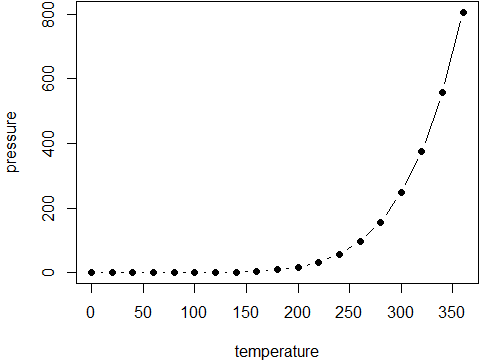
\includegraphics[width=0.8\linewidth]{02-cross-refs_files/figure-latex/nice-fig-1} 

}

\caption{Here is a nice figure!}\label{fig:nice-fig}
\end{figure}

Don't miss Table \ref{tab:nice-tab}.

\begin{Shaded}
\begin{Highlighting}[]
\NormalTok{knitr::}\KeywordTok{kable}\NormalTok{(}
  \KeywordTok{head}\NormalTok{(pressure, }\DecValTok{10}\NormalTok{), }\DataTypeTok{caption =} \StringTok{'Here is a nice table!'}\NormalTok{,}
  \DataTypeTok{booktabs =} \OtherTok{TRUE}
\NormalTok{)}
\end{Highlighting}
\end{Shaded}

\begin{table}

\caption{\label{tab:nice-tab}Here is a nice table!}
\centering
\begin{tabular}[t]{rr}
\toprule
temperature & pressure\\
\midrule
0 & 0.0002\\
20 & 0.0012\\
40 & 0.0060\\
60 & 0.0300\\
80 & 0.0900\\
\addlinespace
100 & 0.2700\\
120 & 0.7500\\
140 & 1.8500\\
160 & 4.2000\\
180 & 8.8000\\
\bottomrule
\end{tabular}
\end{table}

\chapter{Parts}\label{parts}

You can add parts to organize one or more book chapters together. Parts
can be inserted at the top of an .Rmd file, before the first-level
chapter heading in that same file.

Add a numbered part: \texttt{\#\ (PART)\ Act\ one\ \{-\}} (followed by
\texttt{\#\ A\ chapter})

Add an unnumbered part:
\texttt{\#\ (PART\textbackslash{}*)\ Act\ one\ \{-\}} (followed by
\texttt{\#\ A\ chapter})

Add an appendix as a special kind of un-numbered part:
\texttt{\#\ (APPENDIX)\ Other\ stuff\ \{-\}} (followed by
\texttt{\#\ A\ chapter}). Chapters in an appendix are prepended with
letters instead of numbers.

\chapter{Footnotes and citations}\label{footnotes-and-citations}

\section{Footnotes}\label{footnotes}

Footnotes are put inside the square brackets after a caret
\texttt{\^{}{[}{]}}. Like this one \footnote{This is a footnote.}.

\section{Citations}\label{citations}

Reference items in your bibliography file(s) using \texttt{@key}.

For example, we are using the \textbf{bookdown} package
\citep{R-bookdown} (check out the last code chunk in index.Rmd to see
how this citation key was added) in this sample book, which was built on
top of R Markdown and \textbf{knitr} \citep{xie2015} (this citation was
added manually in an external file book.bib). Note that the
\texttt{.bib} files need to be listed in the index.Rmd with the YAML
\texttt{bibliography} key.

The RStudio Visual Markdown Editor can also make it easier to insert
citations:
\url{https://rstudio.github.io/visual-markdown-editing/\#/citations}

\chapter{Blocks}\label{blocks}

\section{Equations}\label{equations}

Here is an equation.

\begin{equation} 
  f\left(k\right) = \binom{n}{k} p^k\left(1-p\right)^{n-k}
  \label{eq:binom}
\end{equation}

You may refer to using \texttt{\textbackslash{}@ref(eq:binom)}, like see
Equation \eqref{eq:binom}.

\section{Theorems and proofs}\label{theorems-and-proofs}

Labeled theorems can be referenced in text using
\texttt{\textbackslash{}@ref(thm:tri)}, for example, check out this
smart theorem \ref{thm:tri}.

::: \{.theorem \#tri\} For a right triangle, if \(c\) denotes the
\emph{length} of the hypotenuse and \(a\) and \(b\) denote the lengths
of the \textbf{other} two sides, we have \[a^2 + b^2 = c^2\] :::

Read more here
\url{https://bookdown.org/yihui/bookdown/markdown-extensions-by-bookdown.html}.

\section{Callout blocks}\label{callout-blocks}

The R Markdown Cookbook provides more help on how to use custom blocks
to design your own callouts:
\url{https://bookdown.org/yihui/rmarkdown-cookbook/custom-blocks.html}

\chapter{Sharing your book}\label{sharing-your-book}

\section{Publishing}\label{publishing}

HTML books can be published online, see:
\url{https://bookdown.org/yihui/bookdown/publishing.html}

\section{404 pages}\label{pages}

By default, users will be directed to a 404 page if they try to access a
webpage that cannot be found. If you'd like to customize your 404 page
instead of using the default, you may add either a \texttt{\_404.Rmd} or
\texttt{\_404.md} file to your project root and use code and/or Markdown
syntax.

\section{Metadata for sharing}\label{metadata-for-sharing}

Bookdown HTML books will provide HTML metadata for social sharing on
platforms like Twitter, Facebook, and LinkedIn, using information you
provide in the \texttt{index.Rmd} YAML. To setup, set the \texttt{url}
for your book and the path to your \texttt{cover-image} file. Your
book's \texttt{title} and \texttt{description} are also used.

This \texttt{gitbook} uses the same social sharing data across all
chapters in your book- all links shared will look the same.

Specify your book's source repository on GitHub using the \texttt{edit}
key under the configuration options in the \texttt{\_output.yml} file,
which allows users to suggest an edit by linking to a chapter's source
file.

Read more about the features of this output format here:

\url{https://pkgs.rstudio.com/bookdown/reference/gitbook.html}

Or use:

\begin{Shaded}
\begin{Highlighting}[]
\NormalTok{?bookdown::gitbook}
\end{Highlighting}
\end{Shaded}

\bibliography{book.bib,packages.bib}

\end{document}
